\documentclass{article}
\setlength{\parskip}{5pt} % esp. entre parrafos
\setlength{\parindent}{0pt} % esp. al inicio de un parrafo
\usepackage{amsmath} % mates
\usepackage[sort&compress,numbers]{natbib} % referencias
\usepackage{url} % que las URLs se vean lindos
\usepackage[top=25mm,left=20mm,right=20mm,bottom=25mm]{geometry} % margenes
\usepackage{hyperref} % ligas de URLs
\usepackage{graphicx} % poner figuras
\usepackage[spanish]{babel} % otros idiomas
\usepackage[utf8]{inputenc} % alparecer son los acentos
\documentclass[12pt,letterpaper]{article}
\usepackage[utf8]{inputenc}
\usepackage{tikz}
\usetikzlibrary{trees}
\usepackage[spanish, es-nodecimaldot]{babel}
\usepackage{color}
\usepackage{algorithm}
\usepackage[noend]{algpseudocode}
\renewcommand{\algorithmicrequire}{\textbf{Entrada:}}
\renewcommand{\algorithmicensure}{\textbf{Salida:}}
\usepackage{subcaption}
\usepackage{amsfonts}
\usepackage{hyperref}
 \hypersetup{
     colorlinks=true,
     linkcolor=blue,
     filecolor=blue,
     citecolor = blue,      
     urlcolor=cyan,
     }
\usepackage{amssymb}
\usepackage{listings}
\usepackage{color}
\author{I E G} % author
\title{Práctica 8: modelo de urnas  } % titulo
\date{\today}

\begin{document} % inicia contenido

\maketitle % cabecera

\begin{abstract} % resumen
En esta práctica \cite{elis8} se simula fenómenos de coalescencia y fragmentación, donde por un lado ciertas partículas se unifican para crear cúmulos más grandes y estos mismos cúmulos se pueden fragmentar para obtener cúmulos más pequeños.
Se supone una cantidad total de $n$ partículas y que al inicio el tamaño de los $k$ cúmulos existentes sigue la distribución normal. Para lograr este fenómeno, se crea $k$ valores de la distribución normal estándar luego normalizamos para convertirlos enteros positivos que sumen $n$ figura \ref{fig1}.

\begin{figure} [h!]% figura
    \centering
    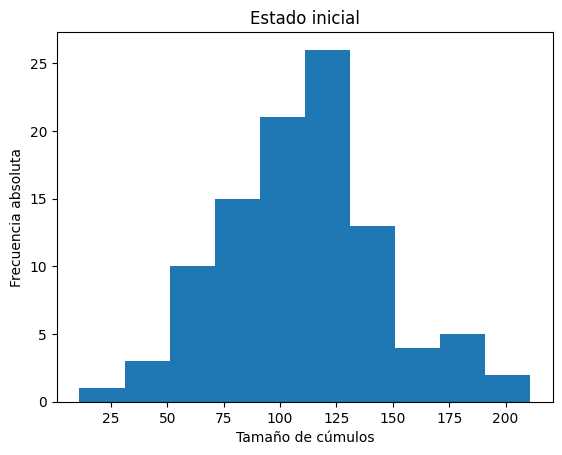
\includegraphics[width=85mm]{fig1.png} % archivo
    \caption{Histograma de normalidad }
    \label{fig1}
\end{figure}

\end{abstract}


\section{Desarrollo}
El desarrollo del código se modifica la codificación en Python de \cite{elis8}\cite{denis2} utilizando una rutina previamente reportada para la creación de los cúmulos, así como la agregación y fragmentación.
La cantidad de cúmulos se varia entre 100, 200 y 400 mientras el número de partículas es de 100000, cada combinación de experimentos se realiza con 15 réplicas.
Al final del el ciclo \cite{cae}, calcula el porcentaje de las partículas filtradas, tomando en cuenta que deben ser mayores al valor critico $c$ y se genera un grafico caja-bigote de los porcentajes de las partículas filtradas. 



\section{Experimento}

Para el experimento \cite{Fab2} se consideran parámetros $k$ que es la cantidad de cúmulos que se tiene y $n$ la cantidad de partículas, el parámetro $k$ varía entre \{100, 200, 400\} figura \ref{fig2}.

\begin{figure} [h!]
 	\centering
 	\begin{subfigure}[b]{0.40\linewidth}
 		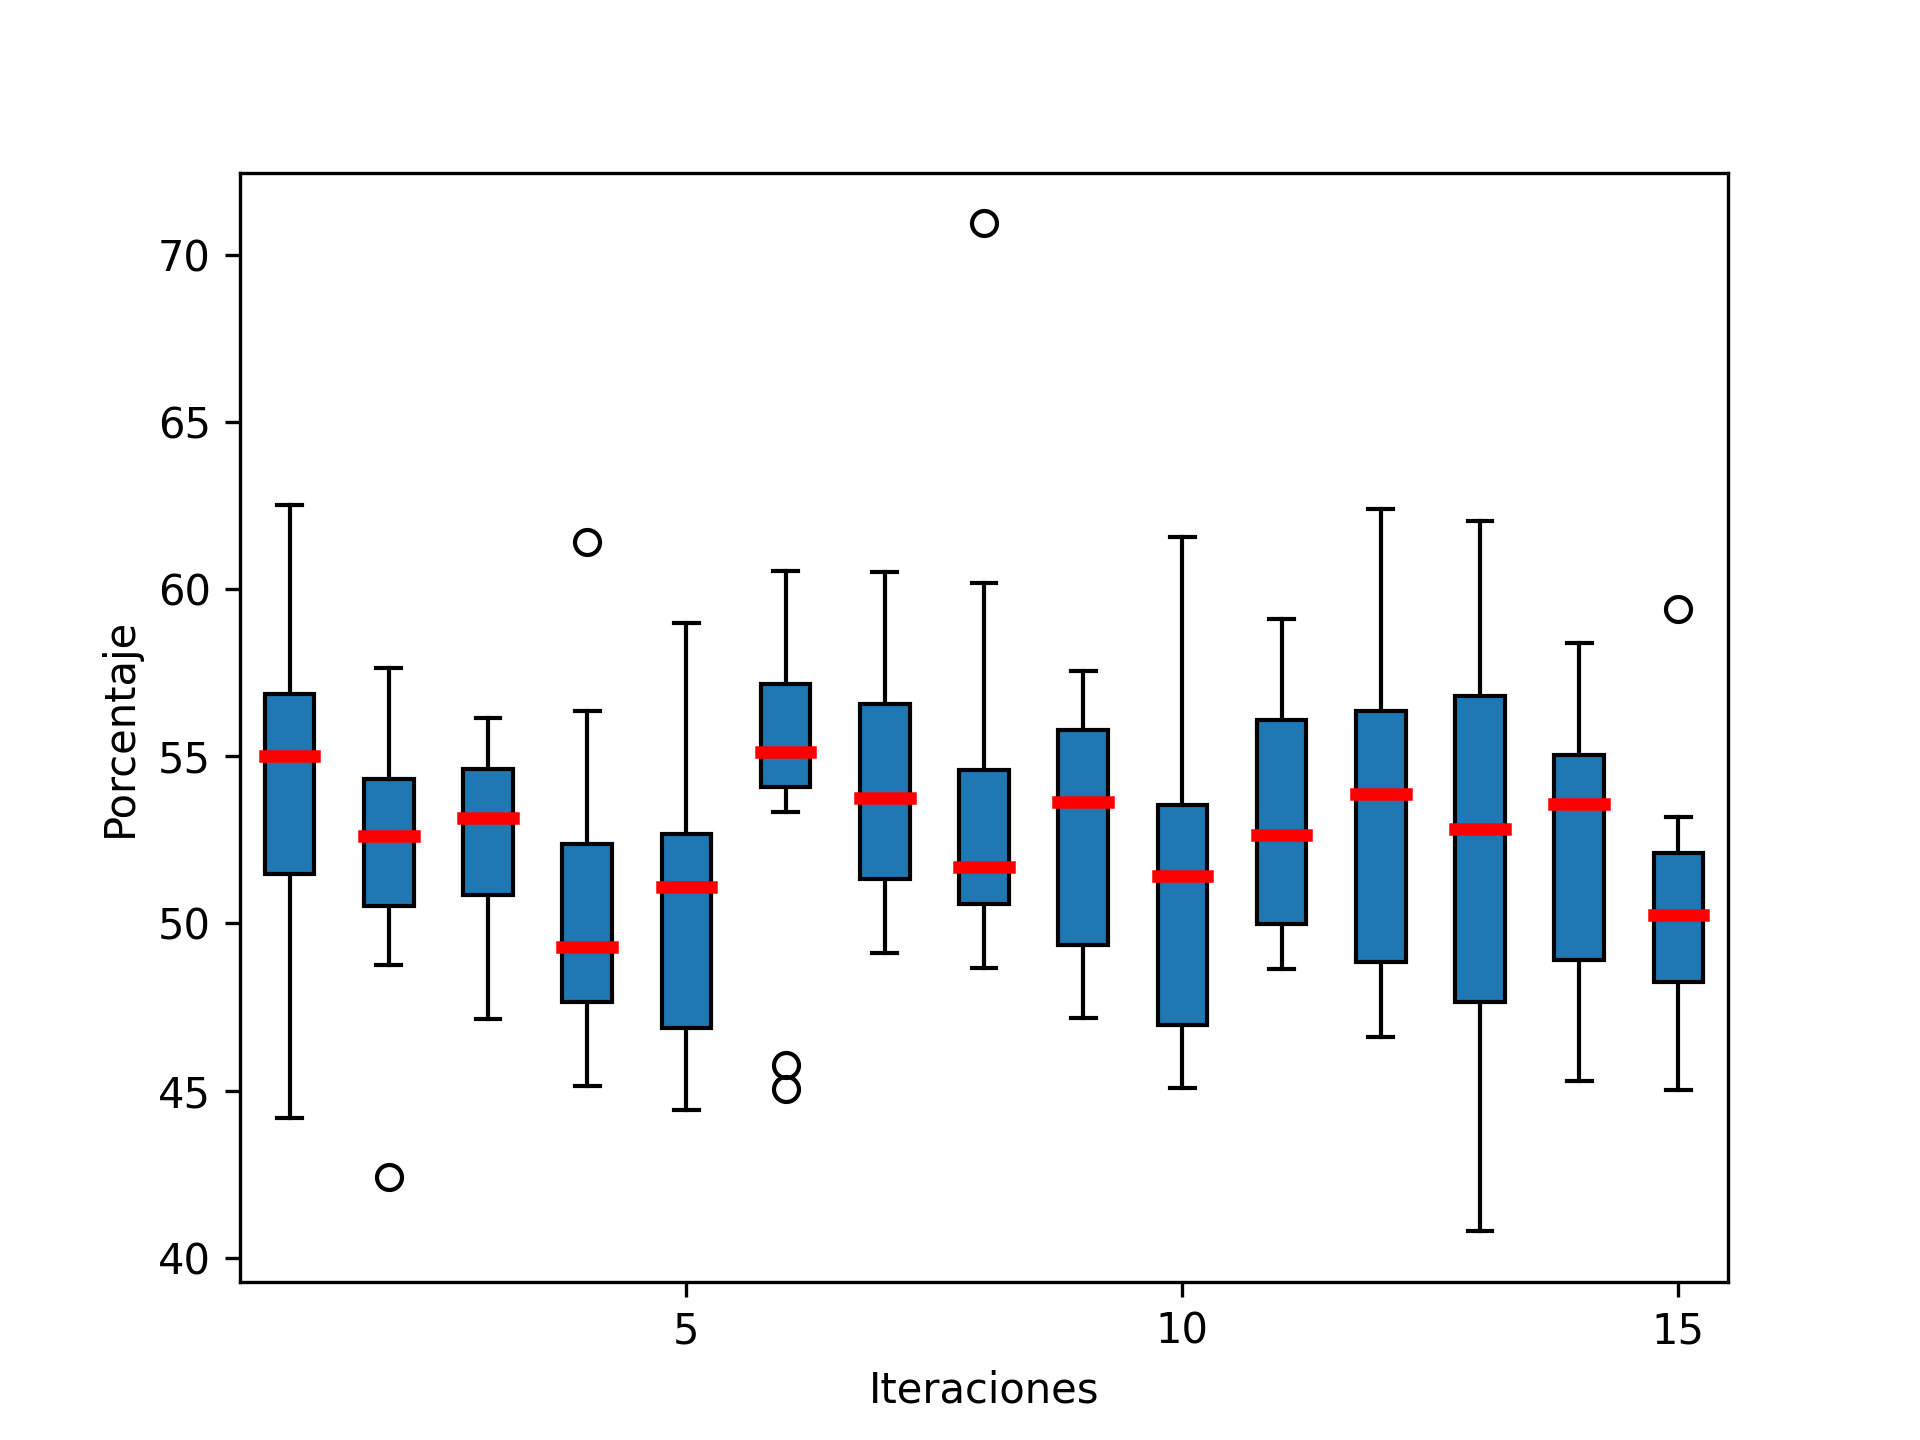
\includegraphics[width=\linewidth]{fig3.png}
 		 \caption{Graficas de caja-bigote con $k$ = 100.}
 		\label{3d}
 	\end{subfigure}
 	\begin{subfigure}[b]{0.40\linewidth}
 		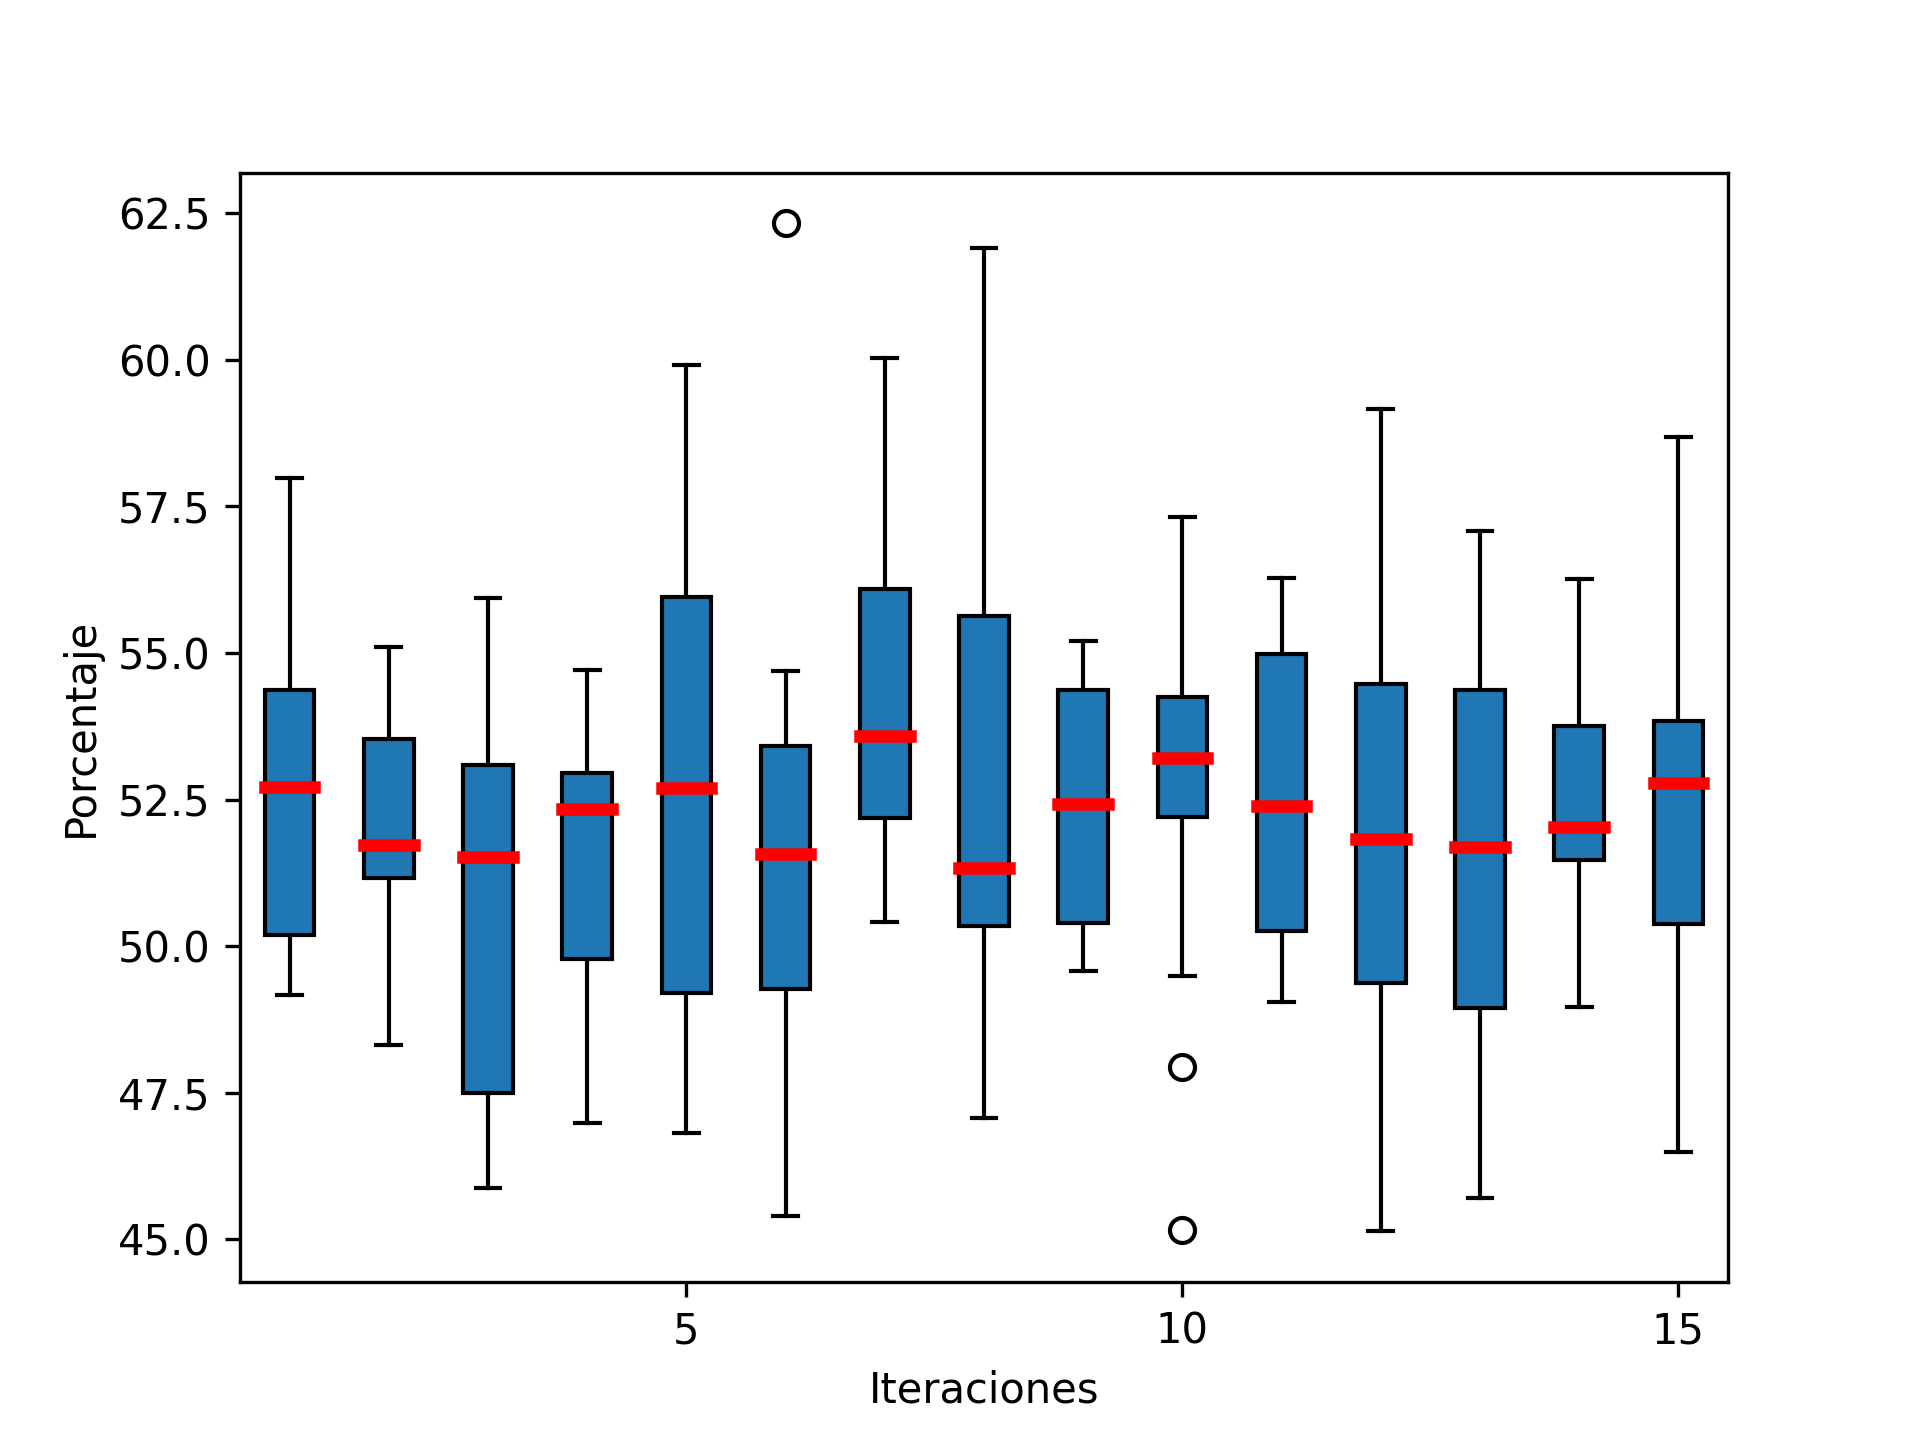
\includegraphics[width=\linewidth]{fig4.png}
 		 \caption{Graficas de caja-bigote con $k$ = 200.}
 		\label{levelplot}
 	\end{subfigure}
 	 	\begin{subfigure}[b]{0.40\linewidth}
 		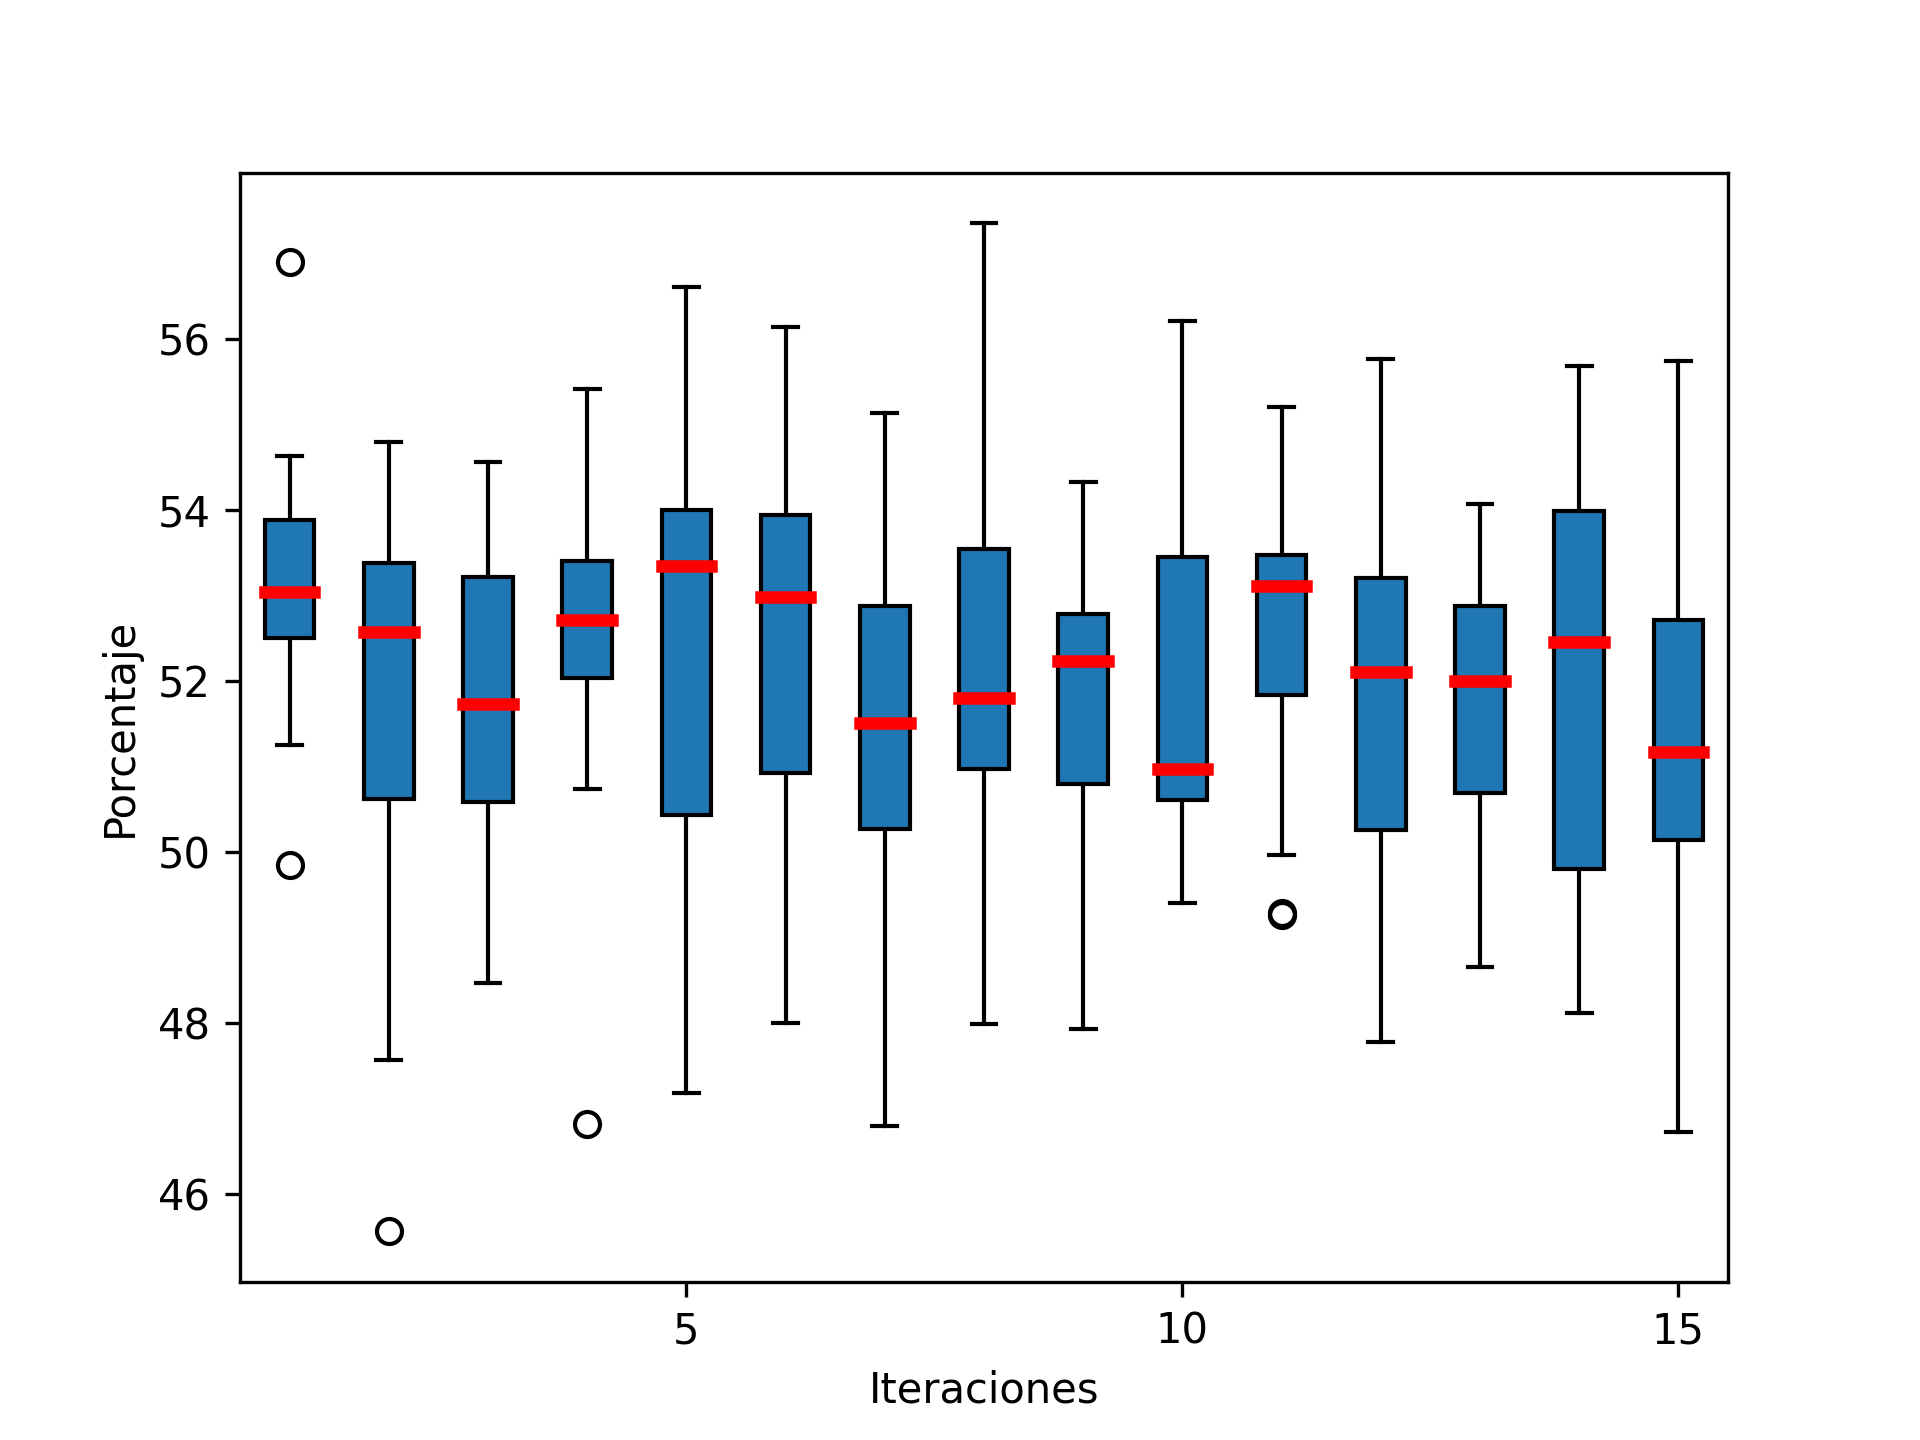
\includegraphics[width=\linewidth]{fig5.png}
 		 \caption{Graficas de caja-bigote con $k$ = 400.}
 		\label{levelplot}
 	\end{subfigure}
 	
 	\caption{experimentacion del porcentaje en gráficas caja-bigote.}  	
\label{fig2}
 \end{figure}
 
\section{Conclusiones} 

La conclusión es que el incremento de la cantidad inicial de partículas aumenta de manera importante el porcentaje de partículas filtradas, mientras que el incremento en la cantidad de cúmulos lo disminuye significativamente como se demuestra en la figura \ref{fig3}.

\begin{figure} [ht]% figura
    \centering
    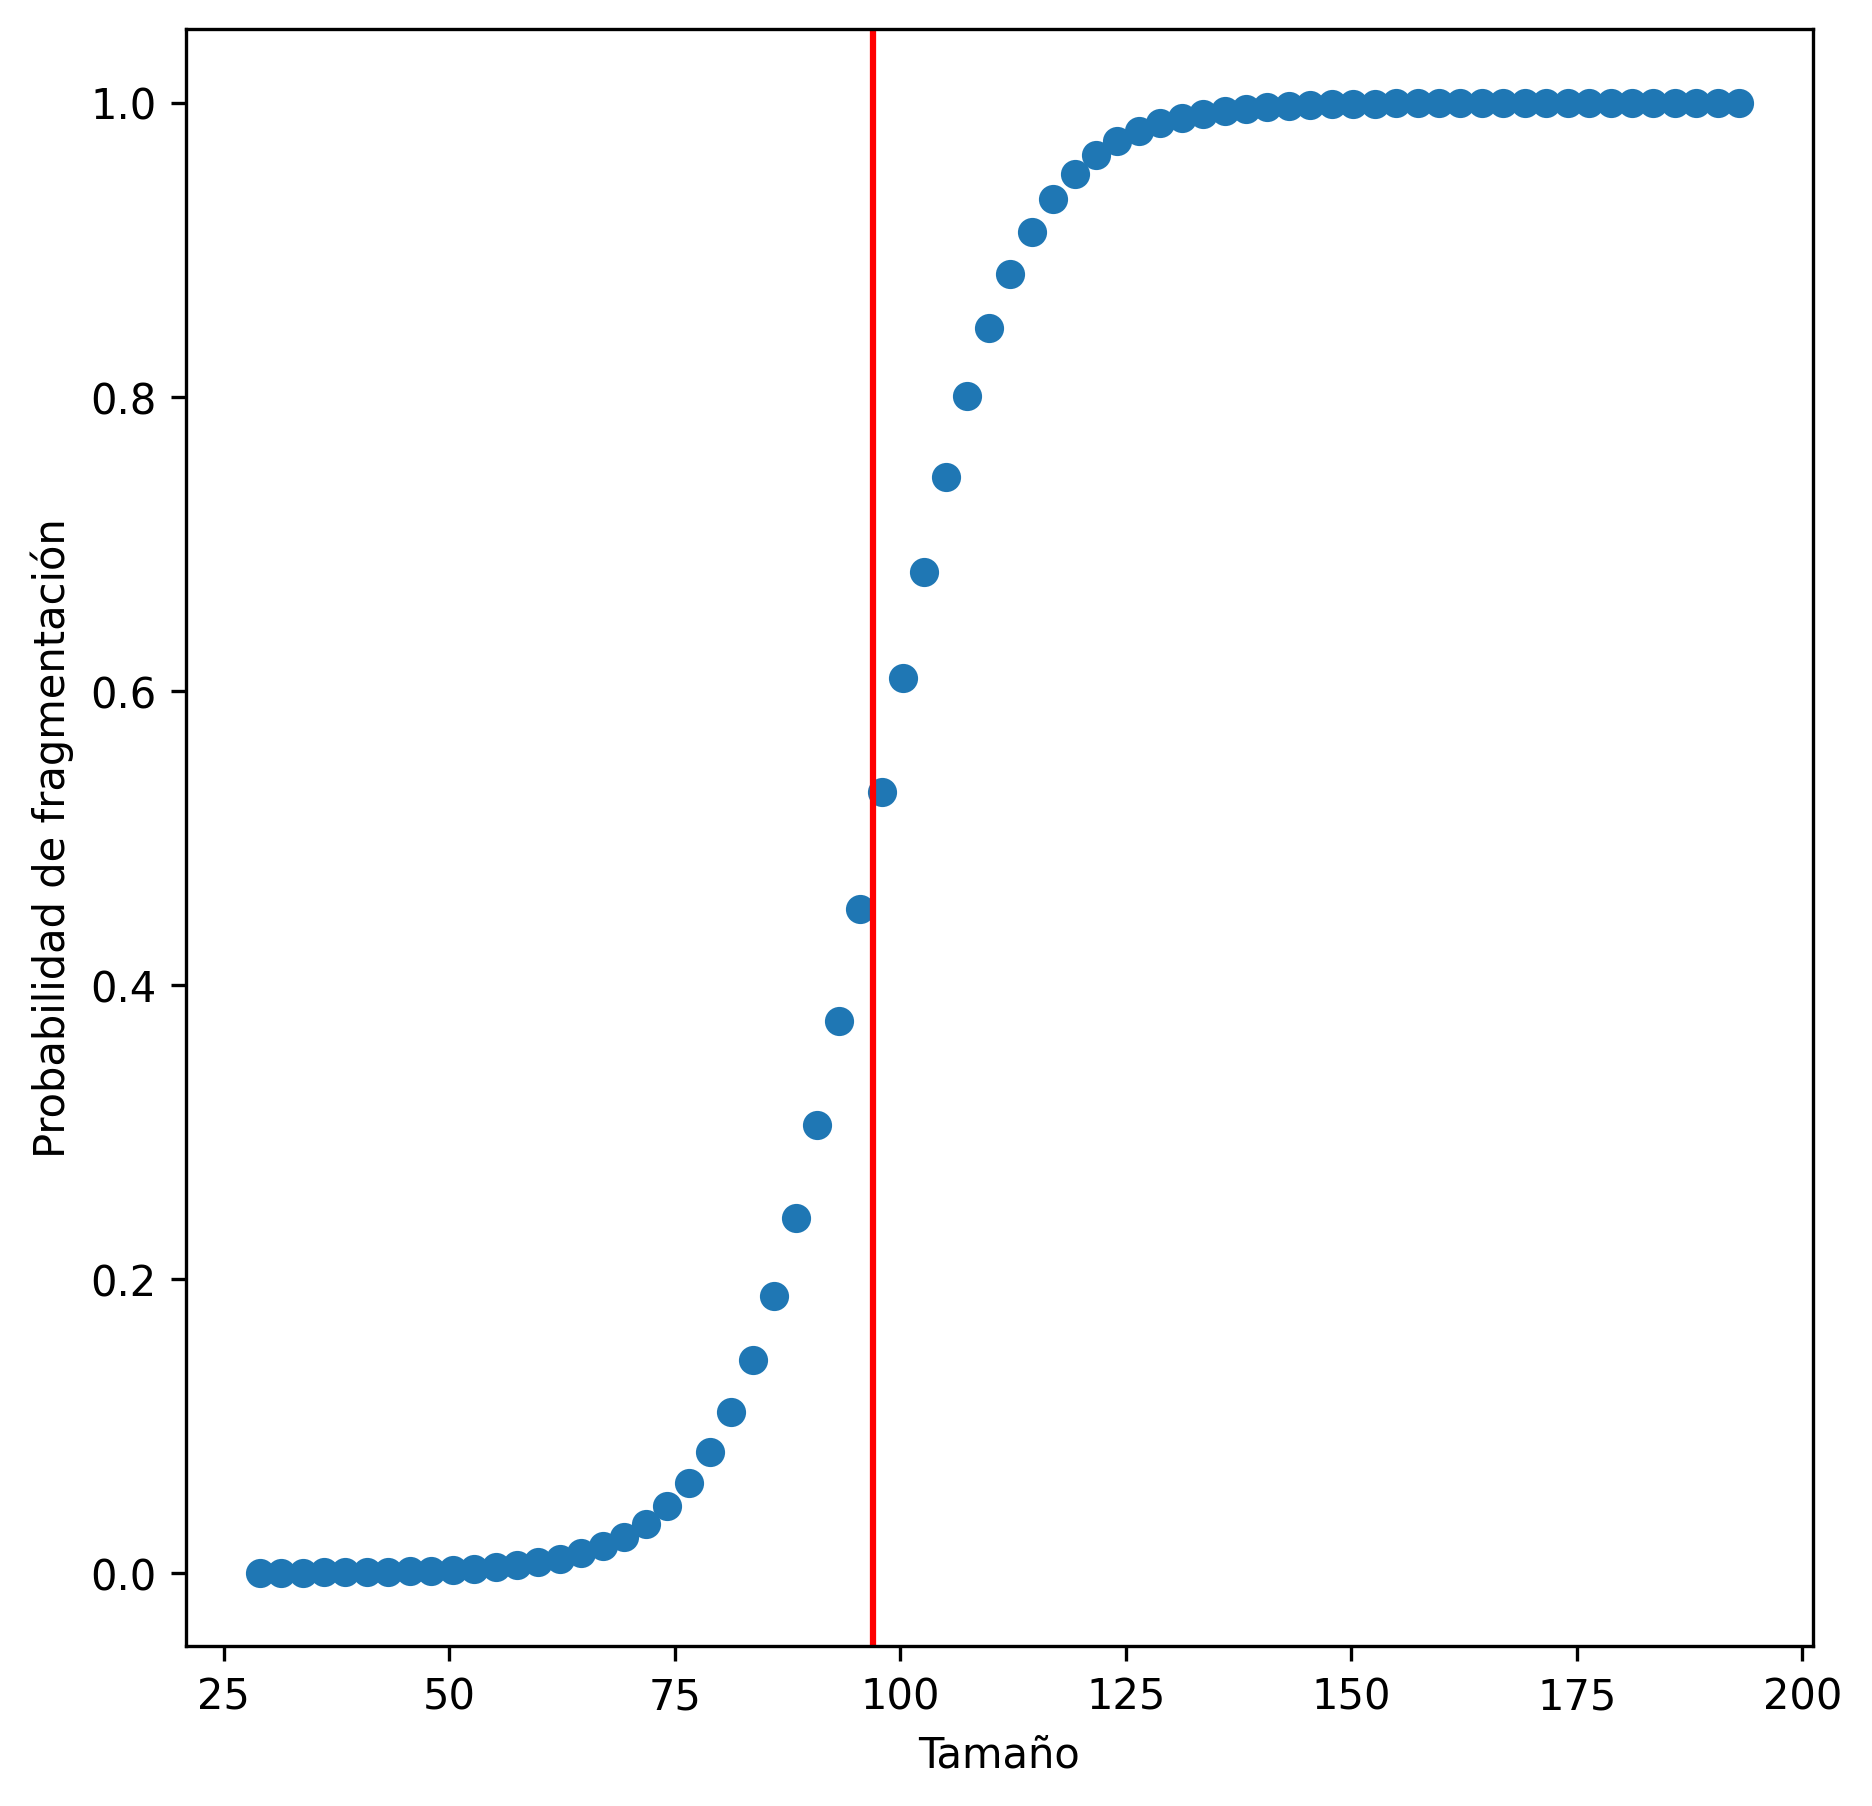
\includegraphics[width=85mm]{fig2.png} % archivo
    \caption{Probabilidad de que un cúmulo con menos de $c$ partículas quiere unirse con otro }
    \label{fig3}
\end{figure}

\bibliography{bib}
\bibliographystyle{plainnat}

\end{document}